\documentclass[aspectratio=169]{beamer}

% ── Theme ──────────────────────────────────────────────────────────────────
\usetheme{Madrid}
\usecolortheme{default}

% ── Custom color palette ────────────────────────────────────────────────────
\definecolor{xaipurple}{RGB}{72,52,120}
\definecolor{xaicyan}{RGB}{0,172,193}
\definecolor{xailight}{RGB}{245,243,255}
\definecolor{xaiaccent}{RGB}{255,112,67}
\definecolor{xaigrey}{RGB}{96,96,108}

\setbeamercolor{palette primary}{bg=xaipurple, fg=white}
\setbeamercolor{palette secondary}{bg=xaipurple!80, fg=white}
\setbeamercolor{palette tertiary}{bg=xaipurple!60, fg=white}
\setbeamercolor{palette quaternary}{bg=xaipurple, fg=white}
\setbeamercolor{structure}{fg=xaipurple}
\setbeamercolor{title}{fg=white, bg=xaipurple}
\setbeamercolor{frametitle}{fg=white, bg=xaipurple}
\setbeamercolor{block title}{bg=xaipurple, fg=white}
\setbeamercolor{block body}{bg=xailight}
\setbeamercolor{block title alerted}{bg=xaiaccent, fg=white}
\setbeamercolor{block body alerted}{bg=xaiaccent!10}
\setbeamercolor{block title example}{bg=xaicyan, fg=white}
\setbeamercolor{block body example}{bg=xaicyan!10}
\setbeamercolor{item}{fg=xaipurple}
\setbeamercolor{subitem}{fg=xaicyan}
\setbeamercolor{subsubitem}{fg=xaiaccent}

% ── Fonts ───────────────────────────────────────────────────────────────────
\usefonttheme{professionalfonts}
\setbeamerfont{title}{size=\Large, series=\bfseries}
\setbeamerfont{frametitle}{size=\large, series=\bfseries}
\setbeamerfont{block title}{series=\bfseries}

% ── Packages ────────────────────────────────────────────────────────────────
\usepackage{amsmath, amssymb}
\usepackage{tikz}
\usetikzlibrary{shapes.geometric, arrows.meta, positioning, shadows}
\usepackage{booktabs}
\usepackage{xcolor}
\usepackage{graphicx}
\usepackage{fontawesome5}
\usepackage{color}
\usepackage{amsopn}
\usepackage{amstext}

% ── Navigation symbols off ──────────────────────────────────────────────────
\setbeamertemplate{navigation symbols}{}

% ── Covered items appear at reduced opacity ──────────────────────────────────
\setbeamercovered{transparent=20}

% ── Section outline ──────────────────────────────────────────────────────────
\AtBeginSection[]{
  \begin{frame}{Outline}
    \tableofcontents[currentsection]
  \end{frame}
}

% ── Custom commands ─────────────────────────────────────────────────────────
\newcommand{\highlight}[1]{\textcolor{xaiaccent}{\textbf{#1}}}
\newcommand{\cyan}[1]{\textcolor{xaicyan}{\textbf{#1}}}

% ── TikZ styles ─────────────────────────────────────────────────────────────
\tikzset{
  box/.style={rectangle, rounded corners=4pt, draw=xaipurple, thick,
              fill=xailight, text width=3.2cm, align=center,
              minimum height=1.1cm, font=\small\bfseries},
  arrow/.style={-Stealth, thick, color=xaipurple},
  methodbox/.style={rectangle, rounded corners=6pt, draw=#1, very thick,
                    fill=#1!12, text width=3.6cm, align=center,
                    minimum height=1.4cm, font=\small},
}

% ────────────────────────────────────────────────────────────────────────────
%  TITLE
% ────────────────────────────────────────────────────────────────────────────
\title[XAI]{Interpretability \& Explainable AI}
\subtitle{From Black Boxes to Transparent Decisions}
\author{Dimitrios Dekas}
\institute{ETH Zurich}
\date{2026}

% ============================================================================
\begin{document}

% ── Title frame ──────────────────────────────────────────────────────────────
\begin{frame}[plain]
  \begin{tikzpicture}[remember picture, overlay]
    \fill[xaipurple] (current page.north west) rectangle (current page.south east);
    \fill[xaicyan!30, opacity=0.4]
      (current page.south west) .. controls +(4,3) and +(-4,2) ..
      (current page.south east) -- (current page.south east) -- cycle;
    \node[white, font=\Huge\bfseries] at ([yshift=1.5cm]current page.center)
      {Interpretability \& XAI};
    \node[white!80, font=\large] at ([yshift=0.5cm]current page.center)
      {From Black Boxes to Transparent Decisions};
    \node[white!60, font=\normalsize] at ([yshift=-0.5cm]current page.center)
      {Dimitrios Dekas};
    \node[white!50, font=\small] at ([yshift=-1.3cm]current page.center)
      {2026};
  \end{tikzpicture}
\end{frame}

% ── Outline ──────────────────────────────────────────────────────────────────
\begin{frame}{Outline}
  \tableofcontents
\end{frame}

% ============================================================================
\section{Why XAI?}
% ============================================================================

\begin{frame}{What is Explainable AI (XAI)?}
  \begin{columns}[T]
    \column{0.47\textwidth}
      \begin{block}<1->{Interpretability}
        \textbf{Intrinsic property}\\[0.4em]
        The model structure is directly human-readable --- no external
        tool needed.\\[0.4em]
        \textit{Examples: linear regression, decision trees}
      \end{block}
    \column{0.47\textwidth}
      \begin{block}<2->{Explainability}
        \textbf{Post-hoc}\\[0.4em]
        A black-box model is described after training via an external
        method.\\[0.4em]
        \textit{Examples: SHAP, LIME, Grad-CAM}
      \end{block}
  \end{columns}
\end{frame}

% ── Interpretability Refresher ────────────────────────────────────────────────
\begin{frame}{Interpretability Refresher}
  \begin{columns}[T]
    \column{0.47\textwidth}
      \begin{block}<1->{Linear Regression}
Each coefficient $\beta_i$ directly quantifies the effect of
        feature $x_i$ on the output. The prediction is a weighted sum
        --- every contribution is explicit and additive.\\[0.4em]
        \textit{$\hat{y} = \beta_0 + \beta_1 x_1 + \cdots + \beta_p x_p$}
      \end{block}
    \column{0.47\textwidth}
      \begin{block}<2->{Decision Trees}
A prediction is produced by following a sequence of
        human-readable if/else rules from root to leaf. The full
        reasoning path is visible and can be stated in plain
        language.\\[0.4em]
        \textit{e.g.\ Age $>$ 30 \& Income $\leq$ 50k $\Rightarrow$ Class A}
      \end{block}
  \end{columns}
\end{frame}

\begin{frame}{Why Does XAI Matter?}
  \begin{block}<1->{Applications}
    \begin{itemize}
      \item \faHospital\ \textbf{Healthcare}
      \item \faChartBar\ \textbf{Finance}
      \item \faCar\ \textbf{Autonomous systems}
      \item Trust, accountability \& safety
      \item Regulatory compliance (e.g.\ GDPR, AI Act)
    \end{itemize}
  \end{block}
  \vspace{0.4em}
  \begin{block}<2->{Technical value}
    \begin{itemize}
      \item \textbf{Debugging}: find data and/or modelling errors
      \item \textbf{Scientific discovery}: gain better insights
    \end{itemize}
  \end{block}
\end{frame}

% ── Shortcut Learning ─────────────────────────────────────────────────────────
\begin{frame}{Why High Accuracy Is Not Enough? Shortcut Learning}
  \begin{alertblock}<1->{Definition}
    A model minimises training loss by relying on features \textbf{irrelevant to
    the true task} --- spurious correlations instead of genuine patterns.
  \end{alertblock}
  \vspace{0.4em}
  \begin{block}<2->{Real-world example}
    \textbf{Skin-cancer classifier}: learned to detect \highlight{ruler marks} in
    dermoscopy images. Rulers appeared more often next to malignant lesions in
    training data.
  \end{block}
  \vspace{0.4em}
  \begin{block}<3->{Takeaway}
    \highlight{High accuracy $\neq$ correct reasoning.}\\
    XAI catches shortcut effects \emph{before} deployment.
  \end{block}
\end{frame}

% ============================================================================
\section{Families of Explainability Methods}
% ============================================================================

\begin{frame}{White-box vs.\ Black-box Models}
  \vspace{-0.2em}
  \begin{columns}[T]
    \column{0.47\textwidth}
      \begin{block}<1->{\faUnlock\ White-box models}
        \begin{itemize}
          \item Structure \& parameters fully \textbf{accessible}
          \item Examples: linear regression, logistic regression, decision trees
          \item Trade-off: typically \emph{less powerful} on complex tasks
          \item Term is sometimes used interchangeably with ``interpretable'' models
        \end{itemize}
      \end{block}
    \column{0.47\textwidth}
      \begin{alertblock}<2->{\faLock\ Black-box models}
        \begin{itemize}
          \item Only input--output behavior exposed
          \item Deep neural networks, proprietary APIs
          \item State-of-the-art performance
          \item Require \textbf{post-hoc} explainability methods
        \end{itemize}
      \end{alertblock}
  \end{columns}
  \vspace{0.5em}
  \begin{exampleblock}<3->{Reality is a spectrum}
    Shallow NNs, regularised ensembles, attention visualization --- occupy an
    \textbf{intermediate} space. The choice involves a practical trade-off between predictive power and understanding.
  \end{exampleblock}
\end{frame}

% ── Local vs Global ───────────────────────────────────────────────────────────
\begin{frame}{Local vs.\ Global Explanations}
  \begin{columns}[T]
    \column{0.47\textwidth}
      \begin{block}<1->{\faSearchLocation\ Local explanations}
        \emph{Why did the model produce \textbf{this} output for \textbf{this} input?}
        \begin{itemize}
          \item Valid only in the neighborhood of one data point
          \item LIME: linear surrogate around a single input
          \item Grad-CAM: per-image heatmap
        \end{itemize}
      \end{block}
    \column{0.47\textwidth}
      \begin{block}<2->{\faGlobe\ Global explanations}
        \emph{What patterns has the model learned \textbf{in general}?}
        \begin{itemize}
          \item Summarise behavior over the full input distribution
          \item Trustworthy regions of model's decision space
          \item Failure mode areas to avoid
          \item Aggregated feature importance rankings
        \end{itemize}
      \end{block}
  \end{columns}
\end{frame}

% ── Four families ─────────────────────────────────────────────────────────────
\begin{frame}{Main Categories of XAI Methods}
  \begin{center}
  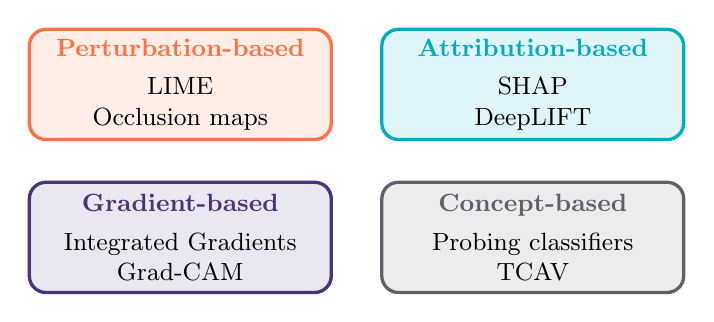
\begin{tikzpicture}[node distance=0.5cm and 0.6cm]
    \node[methodbox=xaiaccent] (pert) {
      \textbf{\textcolor{xaiaccent}{Perturbation-based}}\\[3pt]
      LIME\\Occlusion maps\\[3pt]
    };
    \node[methodbox=xaicyan, right=of pert] (attr) {
      \textbf{\textcolor{xaicyan}{Attribution-based}}\\[3pt]
      SHAP\\DeepLIFT\\[3pt]
    };
    \node[methodbox=xaipurple, below=of pert] (grad) {
      \textbf{\textcolor{xaipurple}{Gradient-based}}\\[3pt]
      Integrated Gradients\\Grad-CAM\\[3pt]
    };
    \node[methodbox=xaigrey, below=of attr] (conc) {
      \textbf{\textcolor{xaigrey}{Concept-based}}\\[3pt]
      Probing classifiers\\TCAV\\[3pt]
    };
  \end{tikzpicture}
  \end{center}
  \vspace{0.3em}
  \begin{exampleblock}{}
    \centering
    All four families are \textbf{complementary} --- use tools from multiple categories.
  \end{exampleblock}
\end{frame}

% ============================================================================
\section{LIME}
% ============================================================================

\begin{frame}{LIME --- Core Idea}
  \begin{block}<1->{Core insight}
    Even if a model is globally complex, its behavior can be approximated
    \highlight{locally} around any input by a simple surrogate model.
  \end{block}
  \vspace{0.5em}
  \begin{block}<2->{Three steps}
    \begin{enumerate}
      \item \textbf{Perturb} the input $x$ to generate $\{z_1,\dots,z_n\}$
      \item \textbf{Query} the black box $f$ and weight by proximity $\pi_x(z_i)$
      \item \textbf{Fit} a simple interpretable surrogate $g^*$ to approximate $f$ locally
    \end{enumerate}
  \end{block}
\end{frame}

\begin{frame}{LIME --- Strengths \& Limitations}
  \begin{exampleblock}<1->{Strengths}
    \begin{itemize}
      \item \textbf{Model-agnostic}: works with any classifier
      \item Applicable across \textbf{images, text, tabular} data
      \item Query-only: works even on proprietary APIs
    \end{itemize}
  \end{exampleblock}
  \vspace{0.5em}
  \begin{alertblock}<2->{Limitations}
    \begin{itemize}
      \item Explanation valid \textbf{only locally}
      \item Quality depends on perturbation strategy
      \item \highlight{Unstable}: running twice may yield different attributions
    \end{itemize}
  \end{alertblock}
\end{frame}

% ============================================================================
\section{SHAP}
% ============================================================================

\begin{frame}{SHAP --- Core Idea}
  \begin{block}<1->{Game-theory foundation}
    Features are \textbf{players}; the model's prediction is the \textbf{payoff}.
    The Shapley value of feature $i$ is its average marginal contribution
    across all possible feature subsets:
    \[
      \phi_i = \sum_{S \subseteq F\setminus\{i\}}
      \frac{|S|!(|F|-|S|-1)!}{|F|!}
      \bigl[f(S\cup\{i\}) - f(S)\bigr]
    \]
  \end{block}
  \vspace{0.4em}
  \begin{block}<2->{Practical variants}
    \begin{description}
      \item[KernelSHAP] LIME-like sampling; provably recovers Shapley values
      \item[TreeSHAP] Exact, polynomial-time for tree-based models
    \end{description}
  \end{block}
\end{frame}

\begin{frame}{SHAP --- Visualisations}
  \begin{columns}[T]
    \column{0.44\textwidth}
      \begin{exampleblock}{Beeswarm plot}
        \begin{center}
        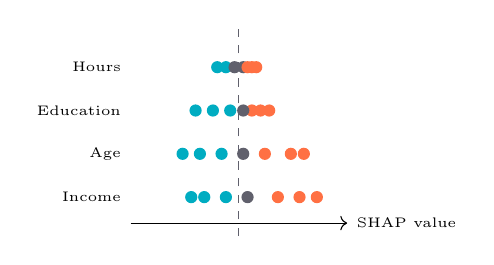
\begin{tikzpicture}[x=0.55cm, y=0.55cm]
          % axes
          \draw[->] (-2.5,0) -- (2.5,0) node[right, font=\tiny]{SHAP value};
          \draw[dashed, xaigrey] (0,-0.3) -- (0,4.5);
          % feature labels
          \foreach \y/\lbl in {0.6/Income, 1.6/Age, 2.6/Education, 3.6/Hours}{
            \node[font=\tiny, anchor=east] at (-2.5,\y) {\lbl};
          }
          % dots per feature (x positions hardcoded for reproducibility)
          % Income
          \foreach \x/\c in {1.8/xaiaccent,1.4/xaiaccent,0.9/xaiaccent,-0.3/xaicyan,-0.8/xaicyan,-1.1/xaicyan,0.2/xaigrey}{
            \fill[\c] (\x,0.6) circle (2.2pt);
          }
          % Age
          \foreach \x/\c in {1.2/xaiaccent,0.6/xaiaccent,-0.4/xaicyan,-1.3/xaicyan,0.1/xaigrey,-0.9/xaicyan,1.5/xaiaccent}{
            \fill[\c] (\x,1.6) circle (2.2pt);
          }
          % Education
          \foreach \x/\c in {0.7/xaiaccent,0.3/xaiaccent,-0.2/xaicyan,-0.6/xaicyan,0.5/xaiaccent,-1.0/xaicyan,0.1/xaigrey}{
            \fill[\c] (\x,2.6) circle (2.2pt);
          }
          % Hours
          \foreach \x/\c in {0.4/xaiaccent,-0.3/xaicyan,0.1/xaigrey,-0.5/xaicyan,0.2/xaiaccent,-0.1/xaigrey,0.3/xaiaccent}{
            \fill[\c] (\x,3.6) circle (2.2pt);
          }
        \end{tikzpicture}
        \end{center}
      \end{exampleblock}
    \column{0.5\textwidth}
      \begin{exampleblock}{Bar chart (mean $|\phi_i|$)}
        \begin{center}
        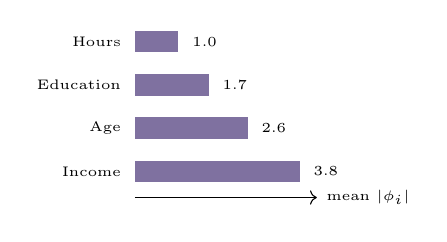
\begin{tikzpicture}[x=0.55cm, y=0.55cm]
          \draw[->] (0,0) -- (4.2,0) node[right, font=\tiny]{mean $|\phi_i|$};
          % bars
          \foreach \len/\y/\lbl in {3.8/0.6/Income, 2.6/1.6/Age, 1.7/2.6/Education, 1.0/3.6/Hours}{
            \fill[xaipurple!70] (0,\y-0.25) rectangle (\len,\y+0.25);
            \node[font=\tiny, anchor=east] at (-0.1,\y) {\lbl};
            \node[font=\tiny, anchor=west] at (\len+0.1,\y) {\len};
          }
        \end{tikzpicture}
        \end{center}
      \end{exampleblock}
  \end{columns}
\end{frame}

% ============================================================================
\section{Grad-CAM}
% ============================================================================

\begin{frame}{Grad-CAM --- Core Idea}
  \begin{block}{Core insight}
    The last convolutional layer retains \textbf{spatial information};
    gradients of the class score $y^c$ w.r.t.\ those feature maps encode
    \highlight{which locations matter most}.
  \end{block}
  \vspace{0.2em}
  \begin{center}
    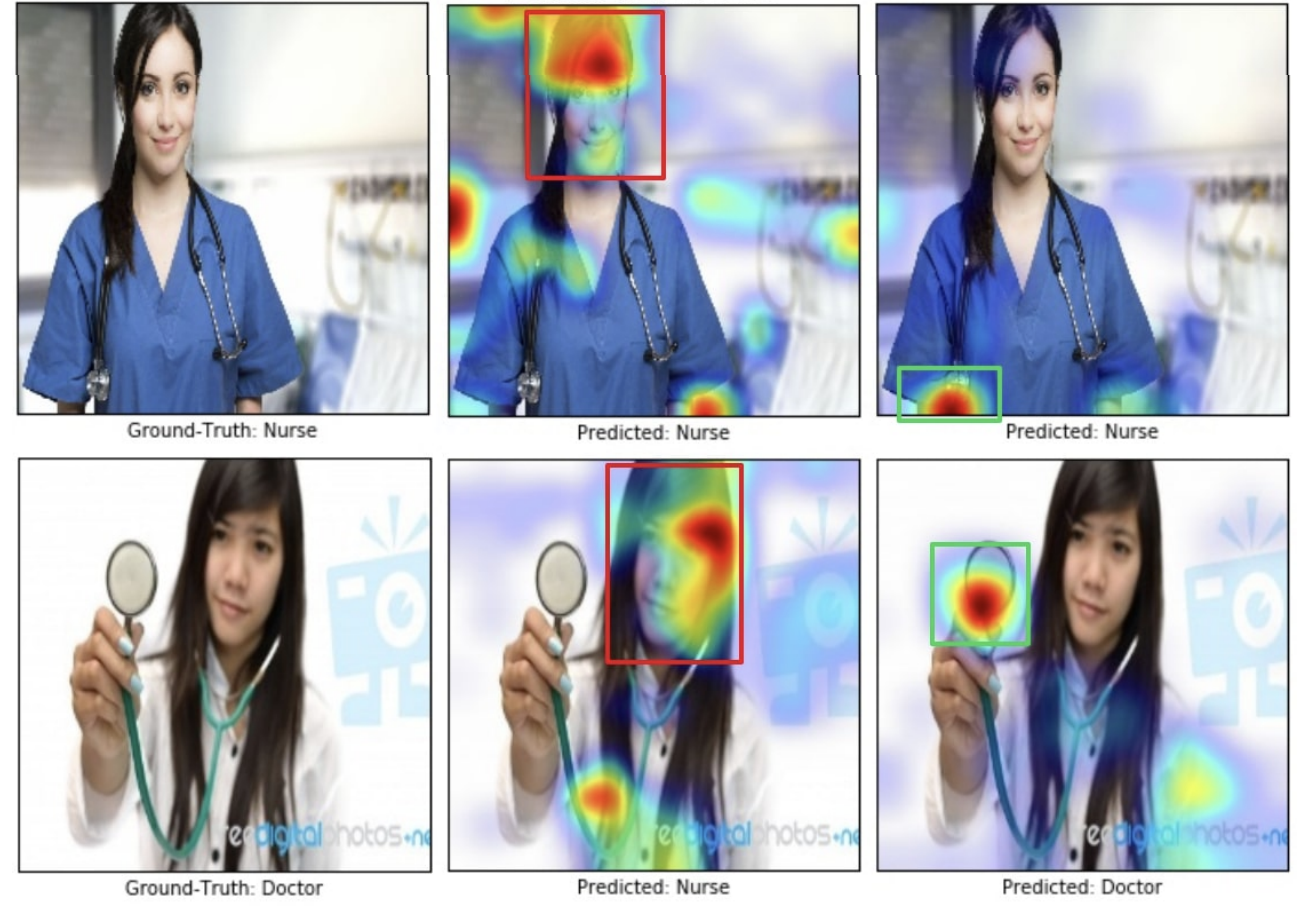
\includegraphics[width=\textwidth, height=0.62\textheight, keepaspectratio]{gradcam_example.png}
  \end{center}
\end{frame}

\begin{frame}{Grad-CAM --- Strengths \& Limitations}
  \begin{exampleblock}<1->{Strengths}
    \begin{itemize}
      \item \textbf{No retraining} required
      \item \textbf{Class-discriminative}: different class $\Rightarrow$ different heatmap
      \item Single forward + backward pass --- \textbf{computationally cheap}
    \end{itemize}
  \end{exampleblock}
  \vspace{0.4em}
  \begin{alertblock}<2->{Limitations}
    \begin{itemize}
      \item Inherits spatial resolution of last conv.\ layer
      \item CNN-specific (not model-agnostic)
    \end{itemize}
  \end{alertblock}
  \vspace{0.4em}
  \begin{block}<3->{Practical use}
    Verify the model attends to the \textbf{right} image regions (stethoscope)
    vs.\ spurious ones (face).
  \end{block}
\end{frame}

% ============================================================================
\section{Probing}
% ============================================================================

\begin{frame}{Probing Classifiers --- Core Idea}
  \begin{block}<1->{What is probing?}
    Train a simple classifier (the \textbf{probe}) on top of a frozen
    intermediate representation to test whether a specific concept is
    \highlight{linearly decodable} from that layer.
  \end{block}
  \vspace{0.4em}
  \begin{block}<2->{Three steps}
    \begin{enumerate}
      \item \textbf{Extract} activations $h^{(\ell)}$ from layer $\ell$ of the
            frozen model for a labelled dataset
      \item \textbf{Train} a lightweight classifier to predict the concept label from $h^{(\ell)}$
      \item \textbf{Evaluate} probe accuracy --- high accuracy $\Rightarrow$
            the concept is encoded in that layer
    \end{enumerate}
  \end{block}
\end{frame}

\begin{frame}{Probing Classifiers --- Strengths \& Limitations}
  \begin{exampleblock}<1->{Strengths}
    \begin{itemize}
      \item Reveals \textbf{what} information is encoded layer-by-layer
      \item Non-invasive: the original model is never modified
      \item Applicable to any architecture that exposes intermediate activations
    \end{itemize}
  \end{exampleblock}
  \vspace{0.4em}
  \begin{alertblock}<2->{Limitations}
    \begin{itemize}
      \item High probe accuracy shows a concept is \emph{present}, not that
            the model \emph{uses} it for its predictions
      \item Results depend on the choice of probe complexity and layer
      \item Requires a labelled concept dataset, which can be costly to obtain
    \end{itemize}
  \end{alertblock}
\end{frame}

% ============================================================================
\section{Summary}
% ============================================================================

\begin{frame}{Summary \& Takeaways}
  \begin{columns}[T]
    \column{0.5\textwidth}
      \begin{block}{The big picture}
        \begin{enumerate}
          \item \highlight{High accuracy is not enough}.
          \item The white-box / black-box distinction determines
                which tools are applicable.
          \item Local \& global explanations are \textbf{complementary}.
          \item Four major families: gradient, perturbation, attribution, concept.
        \end{enumerate}
      \end{block}
    \column{0.45\textwidth}
      \begin{block}{Three workhorse algorithms}
        \begin{center}
        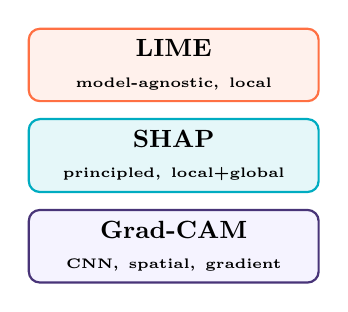
\begin{tikzpicture}[node distance=0.2cm]
          \node[draw=xaiaccent, thick, rounded corners, fill=xaiaccent!10,
                text width=3.4cm, align=center, font=\small\bfseries,
                inner sep=4pt] (l) {LIME\\{\tiny model-agnostic, local}};
          \node[draw=xaicyan, thick, rounded corners, fill=xaicyan!10,
                text width=3.4cm, align=center, font=\small\bfseries,
                inner sep=4pt, below=of l] (s) {SHAP\\{\tiny principled, local+global}};
          \node[draw=xaipurple, thick, rounded corners, fill=xailight,
                text width=3.4cm, align=center, font=\small\bfseries,
                inner sep=4pt, below=of s] (g) {Grad-CAM\\{\tiny CNN, spatial, gradient}};
        \end{tikzpicture}
        \end{center}
      \end{block}
  \end{columns}
  \vspace{0.2em}
  \begin{exampleblock}{\centering Key message}
    \centering
    \textbf{Use XAI not as an afterthought, but as a core part of the ML pipeline}
  \end{exampleblock}
\end{frame}

% ── Thank you ─────────────────────────────────────────────────────────────────
\begin{frame}[plain]
  \begin{tikzpicture}[remember picture, overlay]
    \fill[xaipurple] (current page.north west) rectangle (current page.south east);
    \fill[xaicyan!30, opacity=0.4]
      (current page.north west) .. controls +(4,-3) and +(-4,-2) ..
      (current page.north east) -- (current page.north east) -- cycle;
    \node[white, font=\Huge\bfseries] at (current page.center)
      {Thank you for your attention!};
    \node[white!70, font=\normalsize] at ([yshift=-1cm]current page.center)
      {Questions?};
  \end{tikzpicture}
\end{frame}

\end{document}
